\section{Routing}

\subsection{Background}

For a graph $G=\{V,E\}$ where $O\in V$ is an origin and $D\in V$ is a destination, there is an optimal route $R^* = \{O, \Phi_0, \dots, \Phi_N, D\}| R^*\subset V$ such that $J^*=F(G,R^*)$ is the global minimum value of $J$ for routing cost function $J = F(G,R)$. There are, in essence, two approaches to finding $R^*$, Dijkstra's method and Bellman's method. Both methods are founded on the \gls{hjb} equation

\begin{equation}
	J_k = F(U_k,\dots) + F(U^*_{k+1},\dots)
\end{equation}

which states that the cost of a given control at the current step is the sum of the cost of the control and the cost of the optimal control at the next step subject to the control for a time-varying \gls{ocp}. A corollary is that the optimal control at a given step is influenced by the optimal controls at all following steps. Both Dijkstra's and Bellman's methods work by starting at a given point on a graph with a cost of zero and assigning infinite cost to all other points. The edges of the graph are then explored and for each edge $(u, v)$ if the cost $c(v)$ is greater than the path cost $c(u) + c(u, v)$ then the cost at $v$ is updated to the path cost. This process is called relaxation. The fundamental difference between the methods is that Bellman's method calls for evaluating every edge to check if a relaxation is possible for $|V|$ iterations where $|V|$ is the cardinality of the set of vertices belonging to the graph where Dijkstra's method calls for evaluating only those edges belonging to the "closest" unseen node at each iteration. Dijkstra's method uses a heap queue (priority queue) to keep track of nodes where every node that is reached is added and, at the beginning of each iteration, the edges of node with the smallest cost are evaluated. Essentially, the benefit of Bellman's method over Dijkstra's is that it allows for "upstream" changes to be evaluated constantly where Dijkstra's method only focuses downstream. However Dijkstra's is more often used because it is far more efficient than Bellman's method for the same problem. Generic algorithms can be found in the Appendix. Both methods will usually produce the same globally optimal route. The cases were Bellman's method is needed generally have to do with negative edge costs which are not common in transportation and many other fields. Both methods may be deployed with forward integration (sources to targets) or reverse integration (targets to sources) as diagrammed in Figure \ref{fig:dijkstra}. It is worth noting that \textbf{forward integration creates a tree from a single origin to all destinations} where \textbf{reverse integration creates a tree from all origins to a single destination}. 

\begin{figure}[H]
	\centering
	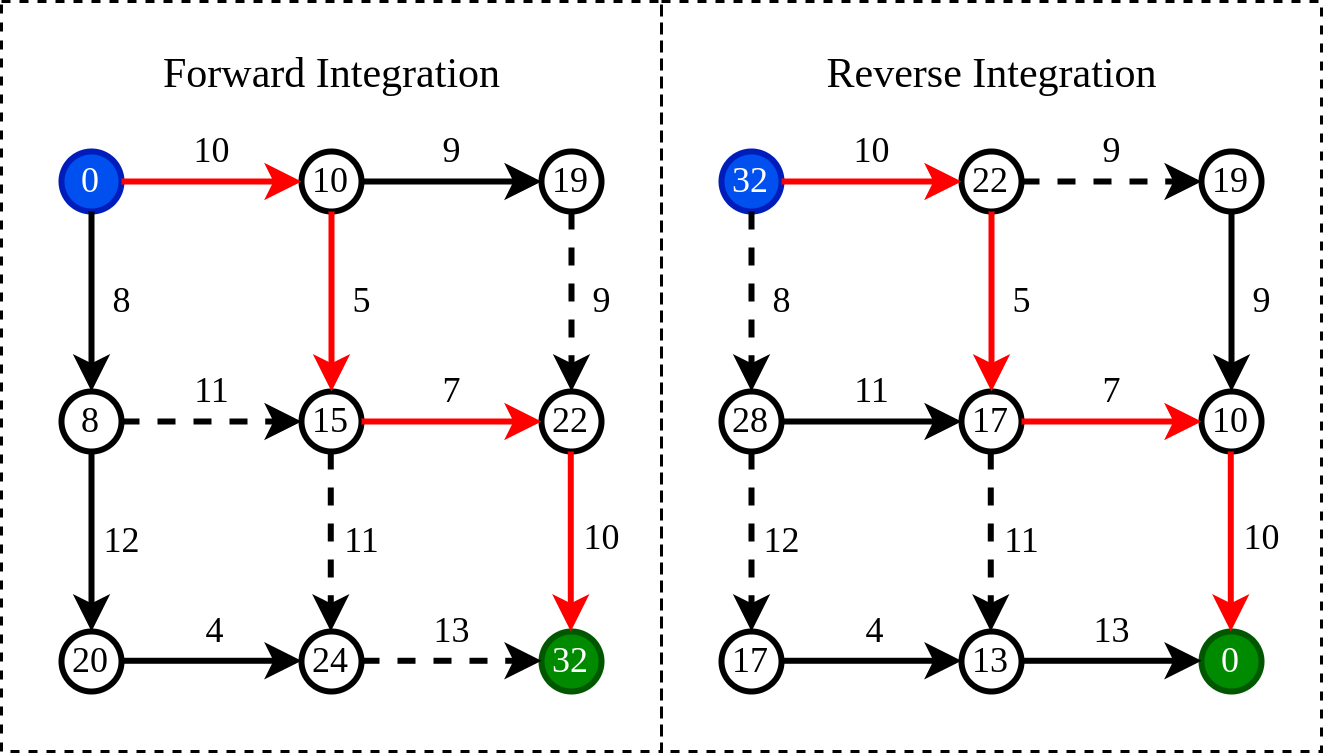
\includegraphics[width = \linewidth]{figs/routing_diagram.png}
	\caption{Comparison between Forward and Reverse Integration for Dijkstra's}
	\label{fig:dijkstra}
\end{figure}


\subsection{Route Constraints}

In the basic formulation presented in the Appendix, minimum cost routes will be found for all destinations. However, in reality, routes can be infeasible for many reasons. Herein two reasons will be focused on these being excessive route cost and insufficient route probability. The cost of a route ($R$) is

\begin{equation}
	J_R = \sum_{v\in V_R}\sum_{f\in F_V} f(v) + \sum_{e\in E_R}\sum_{f\in F_E} f(e)
\end{equation}

where $V_R$ is the set of nodes in $R$, $E_R$ is the set of links connecting $V_R$ in sequence, $F_V$ is the set of cost functions for nodes and $F_E$ is the set of cost functions for links. The probability of route $R$ is

\begin{equation}
	P(R) = \prod_{v\in V_R}P(v) * \prod_{e\in E_R}P(e)
\end{equation}

In general, costs can be either positive or negative and limits on cost can have upper and lower limits. Probabilities for nodes and links will never be less than 0 or more than 1 meaning that increasing route cardinality can only lead to sustained or lowered route probability.

For vehicles, the primary routing constraint will be range. Each vehicle has a limited amount of range and must utilize energizing stations to add range in order to complete certain trips. Graph nodes may be designated as energizing stations. In routing, when an energizing node is reached the vehicle's range is restored and time is added to the route. In this manner, more trips are possible as seen in Figure \ref{fig:routing_chargers}.

\begin{figure}[H]
	\centering
	\begin{subfigure}{.5\linewidth}
		\centering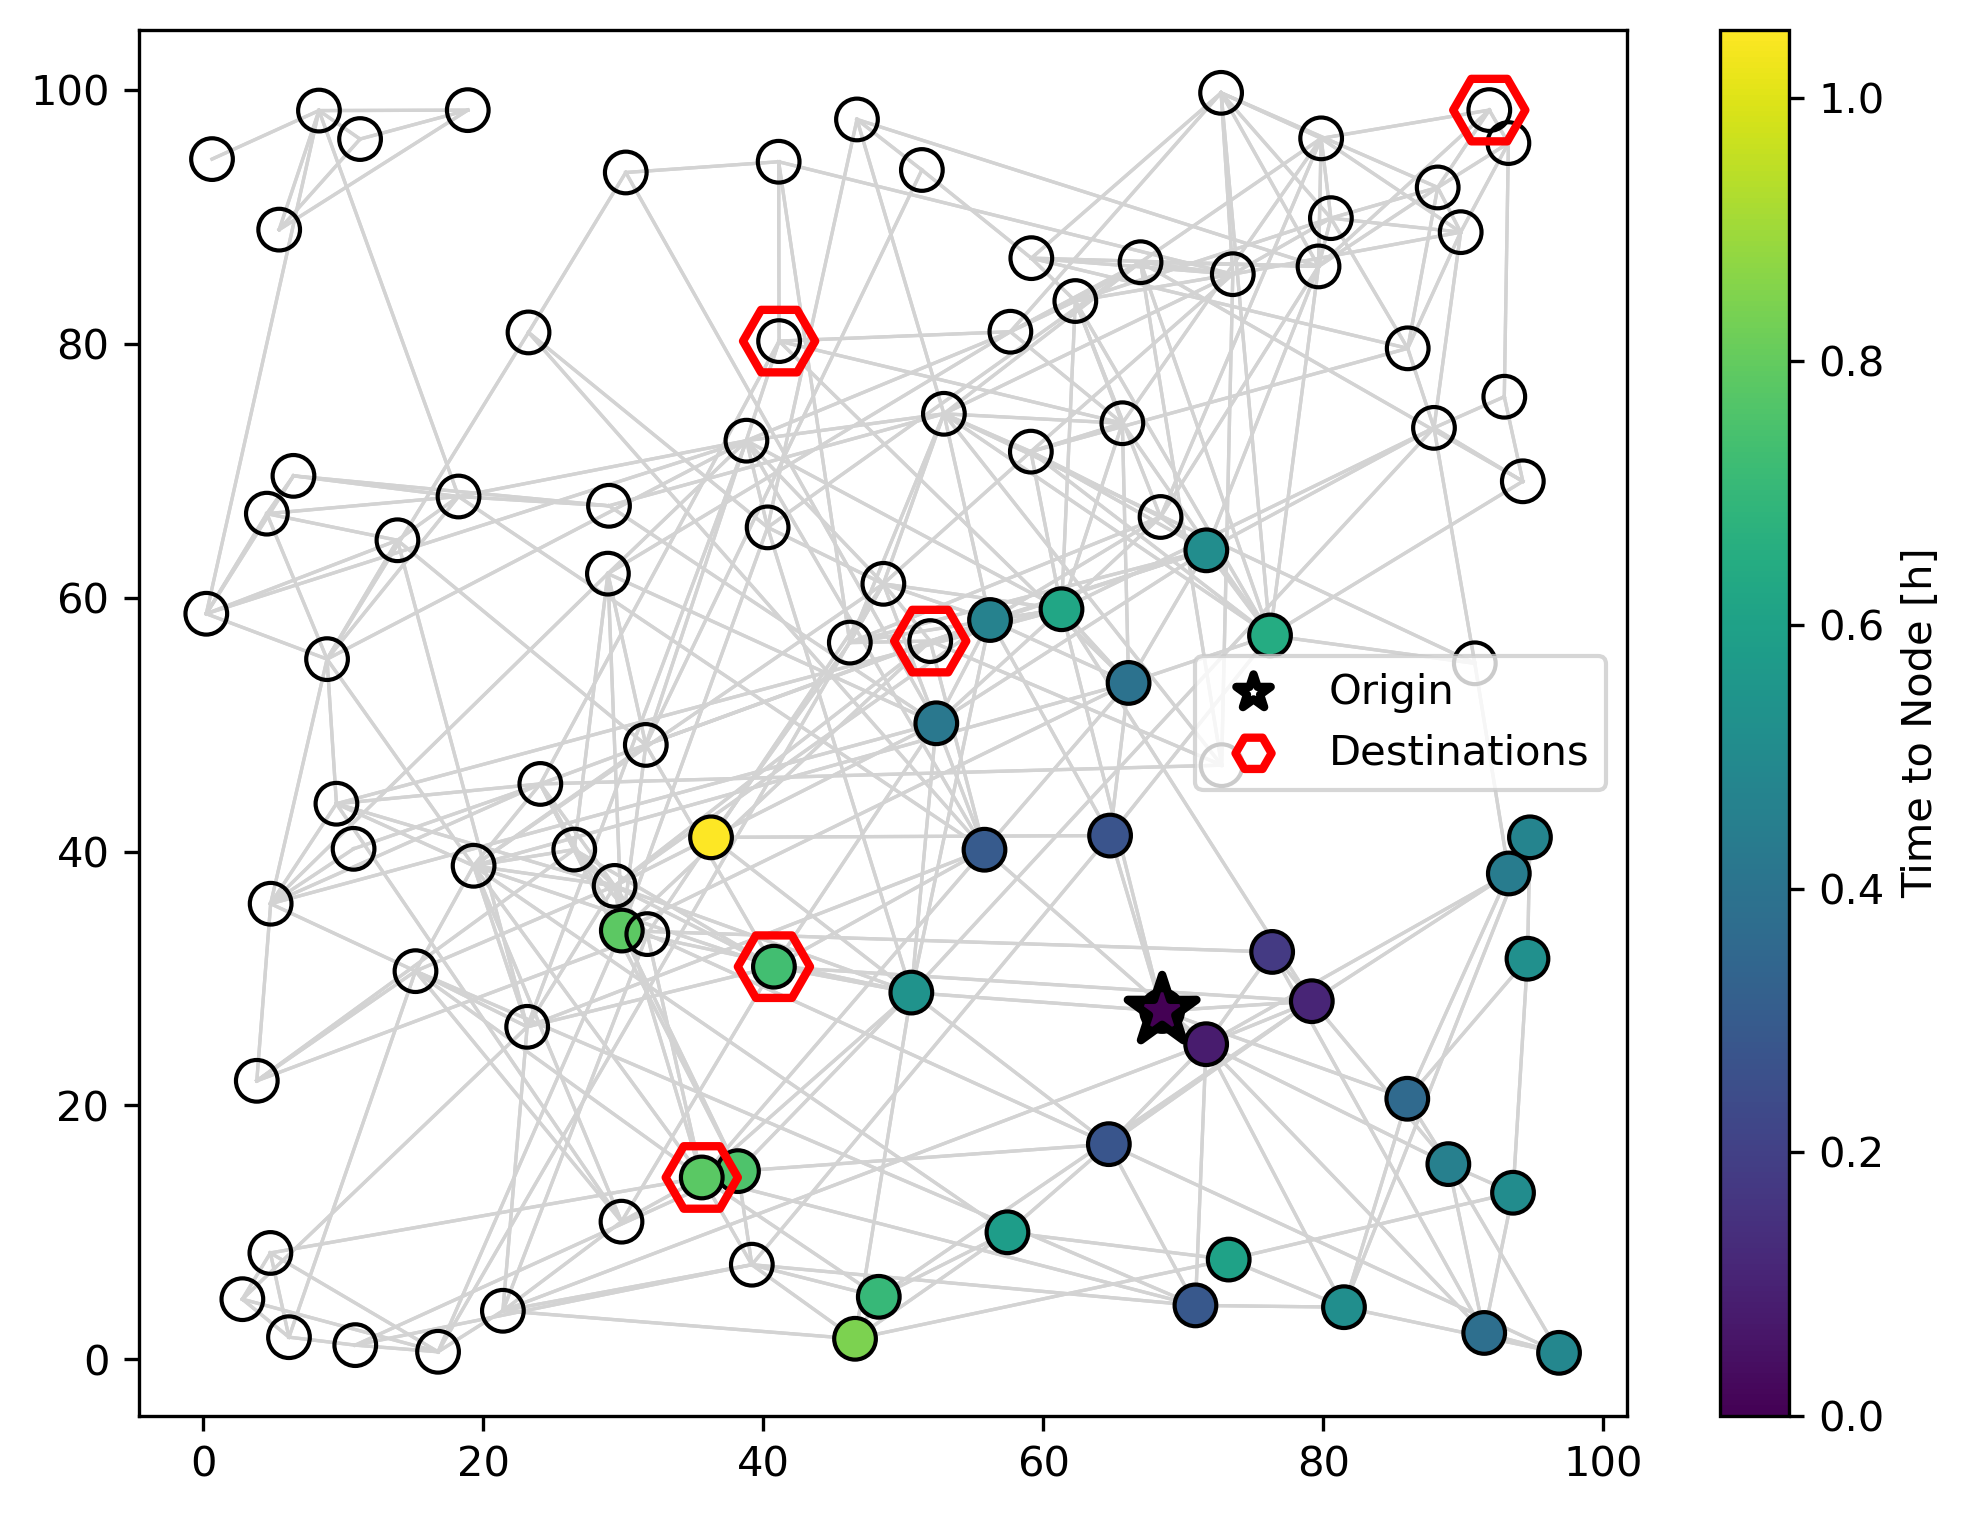
\includegraphics[width = \linewidth]{figs/routing_without_chargers.png}
	\end{subfigure}%
	\begin{subfigure}{.5\linewidth}
		\centering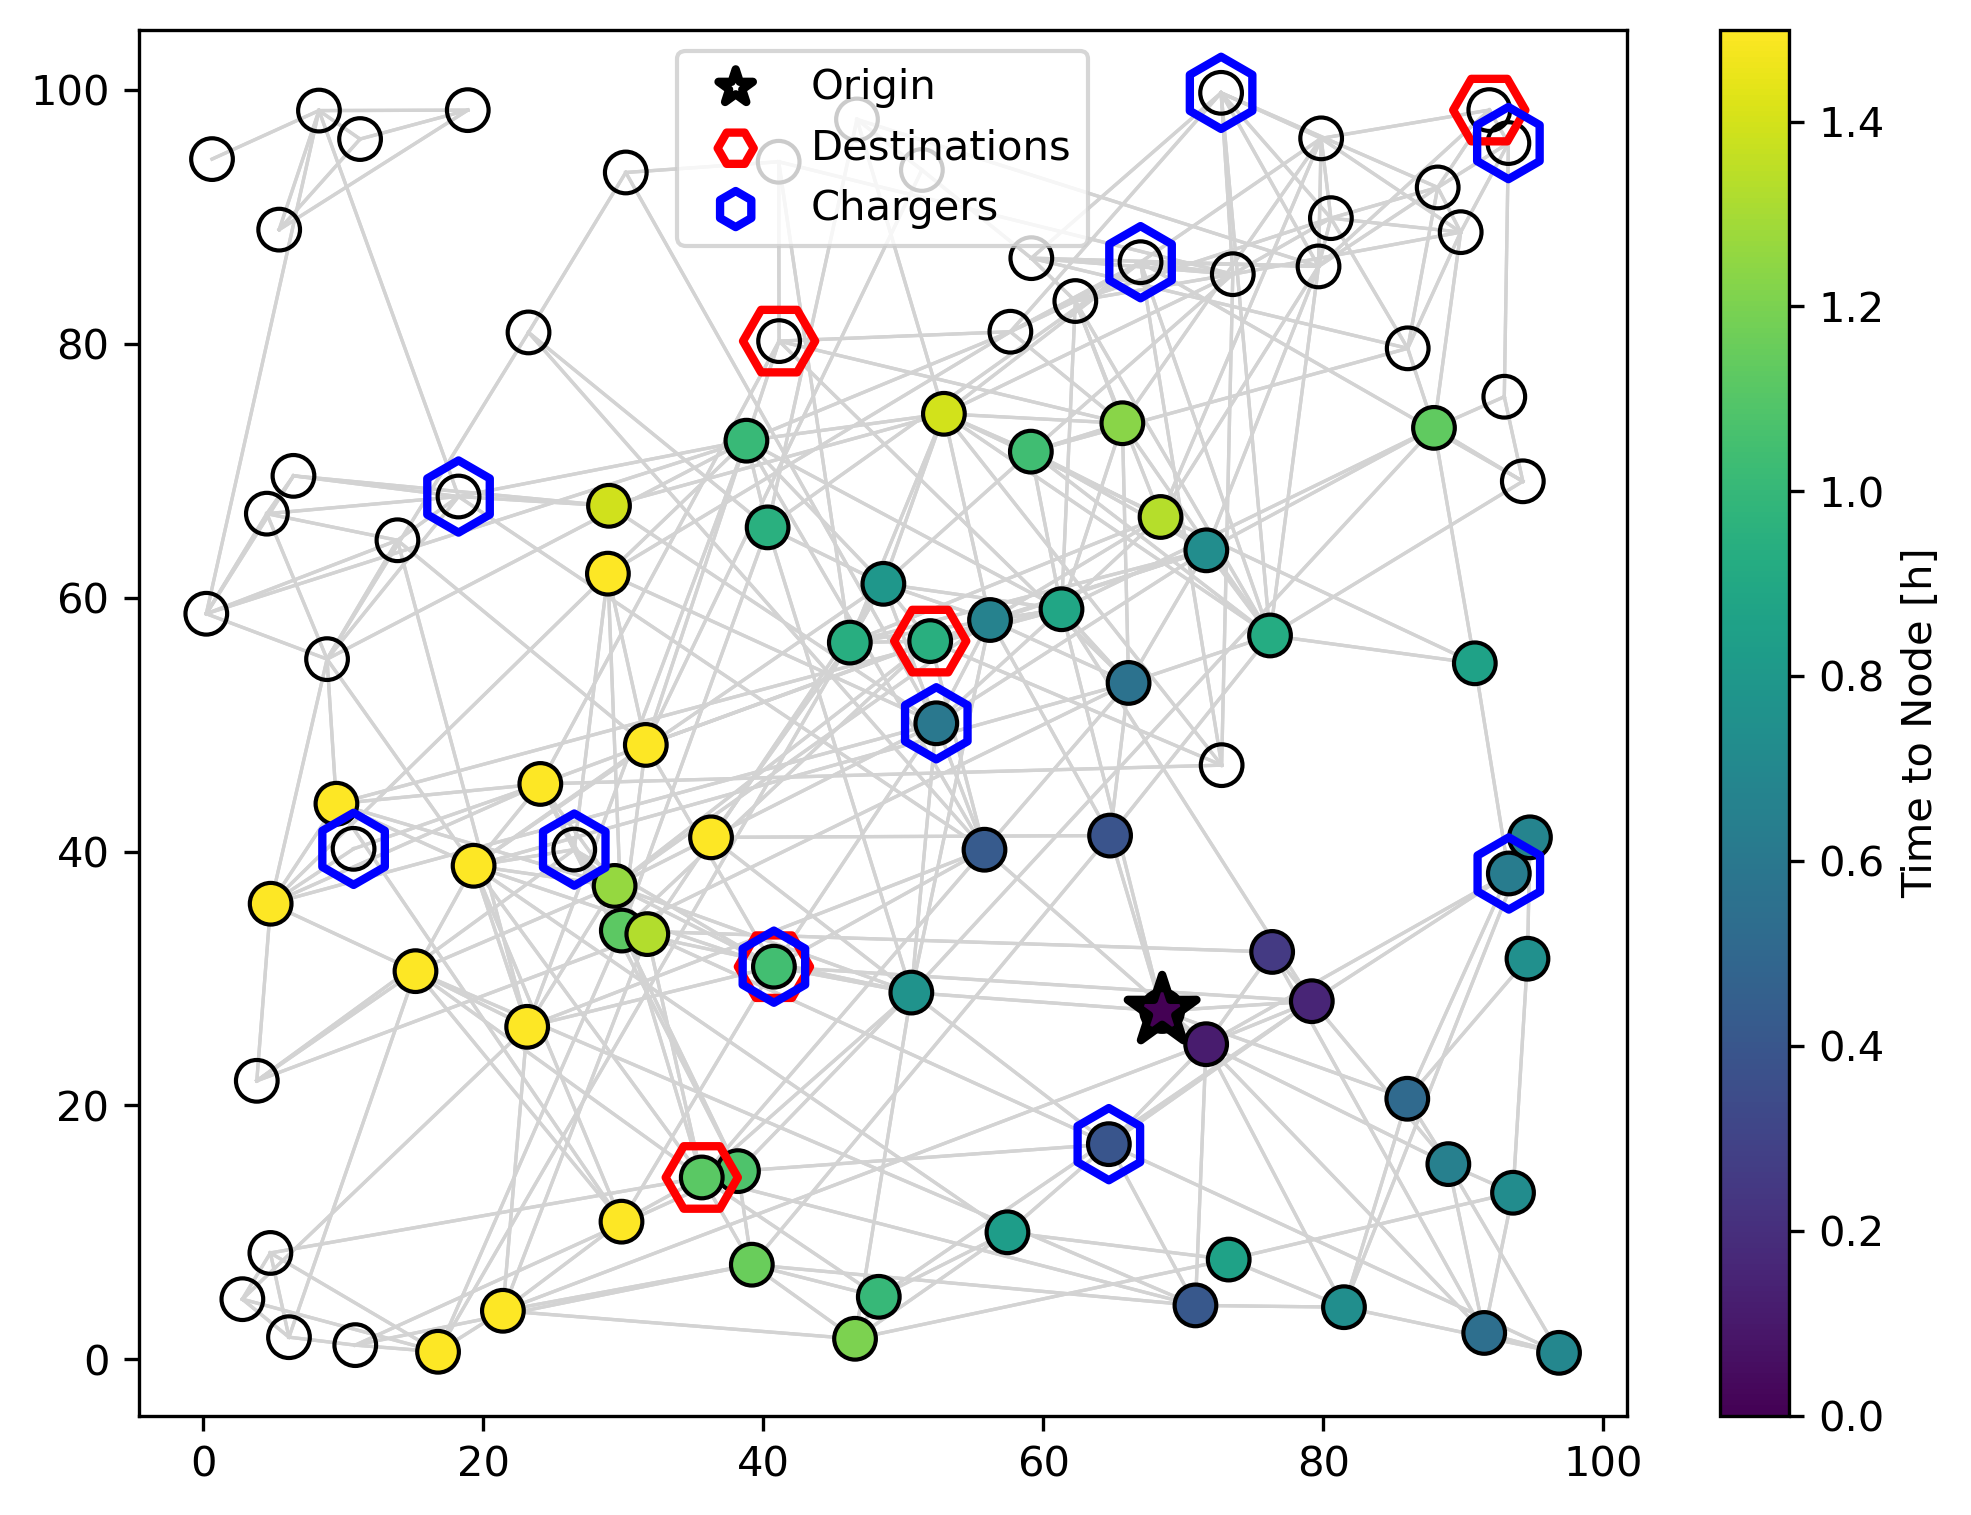
\includegraphics[width = \linewidth]{figs/routing_with_chargers.png}
	\end{subfigure}
	\caption{Routing with (right) and without (left) chargers}
	\label{fig:routing_chargers}
\end{figure}